\documentclass[a4paper, 12pt]{article}

\usepackage{mathtools}

\usepackage{listings}
\usepackage{xcolor}
\usepackage[english]{babel}
\usepackage[labelfont=bf]{caption}
\usepackage[T1]{fontenc}
\usepackage{titlesec, blindtext, color}
\usepackage{float}

\definecolor{gray75}{gray}{0.75}
\newcommand{\hsp}{\hspace{10pt}}
\titleformat{\section}[hang]{\Huge\bfseries}{\thesection\hsp\textcolor{gray75}{|}\hsp}{0pt}{\Huge\bfseries}

\captionsetup{labelfont=bf}

\definecolor{codegreen}{rgb}{0,0.6,0}
\definecolor{codegray}{rgb}{0.5,0.5,0.5}
\definecolor{codepurple}{rgb}{0.58,0,0.82}
\definecolor{backcolour}{rgb}{0.95,0.95,0.95}

\lstdefinestyle{mystyle}{
    backgroundcolor=\color{backcolour},   
    commentstyle=\color{codegreen},
    keywordstyle=\color{blue},
    numberstyle=\tiny\color{codegray},
    stringstyle=\color{orange},
    basicstyle=\ttfamily\footnotesize,
    breakatwhitespace=false,         
    breaklines=true,                 
    captionpos=b,                    
    keepspaces=true,                 
    numbers=left,                    
    numbersep=5pt,                  
    showspaces=false,                
    showstringspaces=false,
    showtabs=false,                  
    tabsize=2
}

\lstset{style=mystyle}

\includeonly{
    chapters/introduction,
    chapters/architecture,
    chapters/vhdl_code,
    chapters/test_plan,
    chapters/xilinx_report,
    chapters/conclusion 
}



\begin{document}
\begin{titlepage}
    \begin{center}
        \begin{figure}
            
\includegraphics[width=\textwidth]{img/marchio_unipi_pant541-eps-converted-to.pdf}         
        \end{figure}
        {\Large
        Computer Engineering\\
        \vspace{5mm} %5mm vertical space
        Electronic and Communication Systems}\\
        \vspace{30mm} %5mm vertical space
        {\Huge\textbf{\textit{Perceptron}}}\\
        \vspace{10mm} %5mm vertical space
        {\Large Project Report}\\
        \par\noindent\rule{\textwidth}{0.4pt}
            \begin{flushright}
                \textit{TEAM MEMBERS}:\\
                Olgerti Xhanej\\
            \end{flushright}
            \vfill
        Academic Year: 2020/2021\\        
    \end{center}
\end{titlepage}    
\tableofcontents

\section{Introduction}
\subsection{Problem Description}
The main goal of the activity described in this report is the following: realizing a network implementing a \textbf{perceptron} with a \textbf{sigmoid activation function}.\\
Before describing the whole design and implementation process a very little introduction about the architecture must be done.\\

\begin{figure}[h]
	\centering
	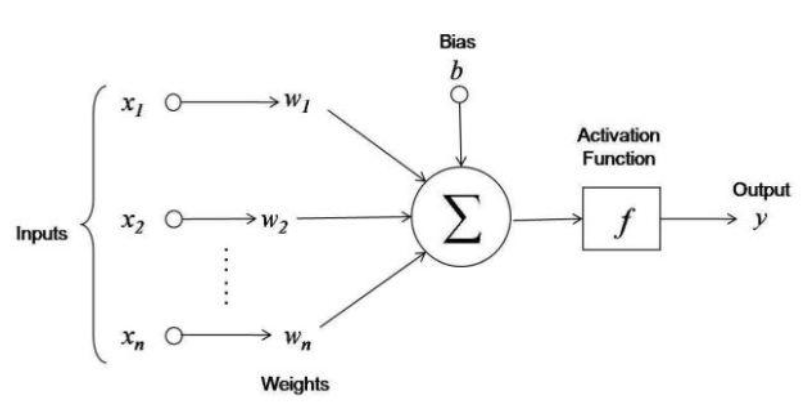
\includegraphics[width=\textwidth]{img/perceptron.png}
	\caption{Perceptron Architecture}
\end{figure}

A \textbf{Perceptron} is a \textit{binary classifier that maps his inputs to a specific output y = f(z), where f() is the \textbf{activation function} of the perceptron.} The inputs are real numbers and the input z of the activation function is obtained as:\\
\begin{equation}
	z = b + \sum_{i = 0}^{N_{L}-1}w_{i}x_{i}
\end{equation}

Every input $x_{i}$, every weight $w_{i}$ and the bias $b$ are real numbers in the range of $[-1, 1]$. \\
The \textbf{activation function}, in our case, will be a \textbf{sigmoid function}, described as follows:
\begin{figure}[h]
	\centering
	\caption{Sigmoid Function Plot}
	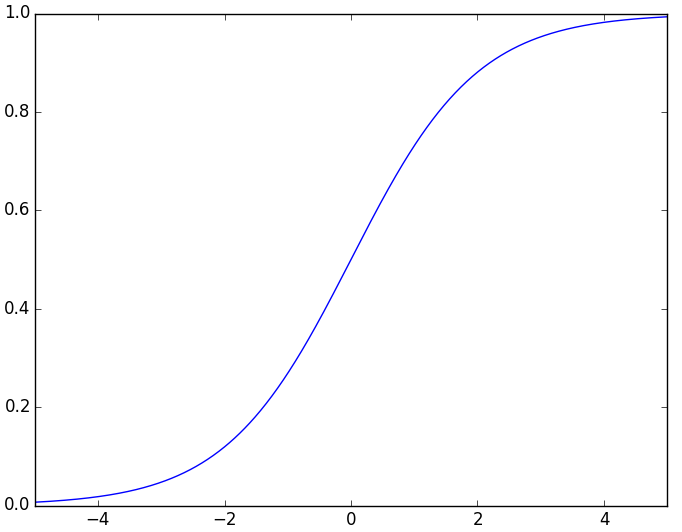
\includegraphics[width=8cm]{img/sigmoid.png}
\end{figure}
\begin{equation}
	y = \dfrac{1}{1+e^{-z}}
\end{equation}
Where $z$ is the result of the equation (1.1).
\subsection{Applications}
A single perceptron is the building block of \textit{artificial neural networks}, in which different layers of perceptrons are connected. The output of the neural network is a real number and could be use to classify \textit{complex objects}: patterns, human faces, handwritings, medical diagnosis, e-mail spams.\\
\begin{figure}[H]
	\centering
	\caption{Neural network example}
	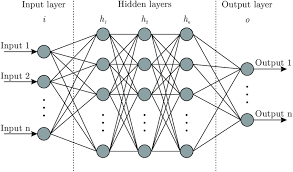
\includegraphics[width=8cm]{img/neural_network.png}
\end{figure}
In the image above there is a simple schema of a neural network, in which the circles represent the perceptrons.
\subsection{Possible Architectures}

The main architecture will be made up by three main logical parts, from an higher-lever point of view:
\begin{itemize}
	\item \textbf{Multiplication Circuit}: implementation of the multiplication operation between each input $x_{i}$ and each weight $w_{i}$.
	\item \textbf{Adder Circuit}: implementation of the addition between the results of the former phase and the bias $b$.
	\item \textbf{Activation Function Circuit}: implementation of the computation of the sigmoid function.
\end{itemize}

In the next chapter the architecture will be documented with more precision.
Different project choices could be made for each logical part of the architecture:

\begin{itemize}
	\item{\textbf{Multiplication Circuit}}: could be implemented through a \textbf{ROM-based solution} in which every possible result is stored and the two inputs represent the addresses for getting the result. This solution is good only with a very low number of bits, which is not our case: in fact the the ROM will be composed by $2^{(n_{w_{i}} + n_{b_{i}})}$ memory cells. In order to implement the multiplication circuit will be implemented through a  \textbf{Paraller Multiplier}.
	\item{\textbf{Adder Circuit}}: different choice could be made to implement the adder circuit. Starting from the simplest to the more complex solution we can exploit the \textbf{Serial Adder}, the \textbf{Parallel Adder} or the \textbf{Parallel Adder with Pipeline }. The first one needs less logic but requires $n$ clock cycles for computing an $n$ bits result. The second solution improves the first one by computing one result in \textbf{one clock cycle}, on the other hand it could add some problems due to long logic chains between two register. The third solution is the best from the perspective of the number of clock cycles required and the \textbf{critical path}, in fact by adding some registers in between the computation of the bits will reduce the logic chains. 
	\item{\textbf{Activation Function Circuit}}: As seen during the laboratory class, this part will be implemented by exploiting a Look-Up-Table. In order to do so, could be necessary a \textbf{truncation} of the result of the former computation in order to limit the size of the LUT. With $12$ bits are necessary $2^{12} = 4096$ entries, which could be even reduced by performing some optimization by exploiting the sigmoid function symmetry.
\end{itemize} 

\section{Architecture}

In this chapter will be discussed deeply the architecture of the three main parts of the \textbf{Perceptron}. The general structure could be summarized by the following schema:
\begin{figure}[H]
	\centering
	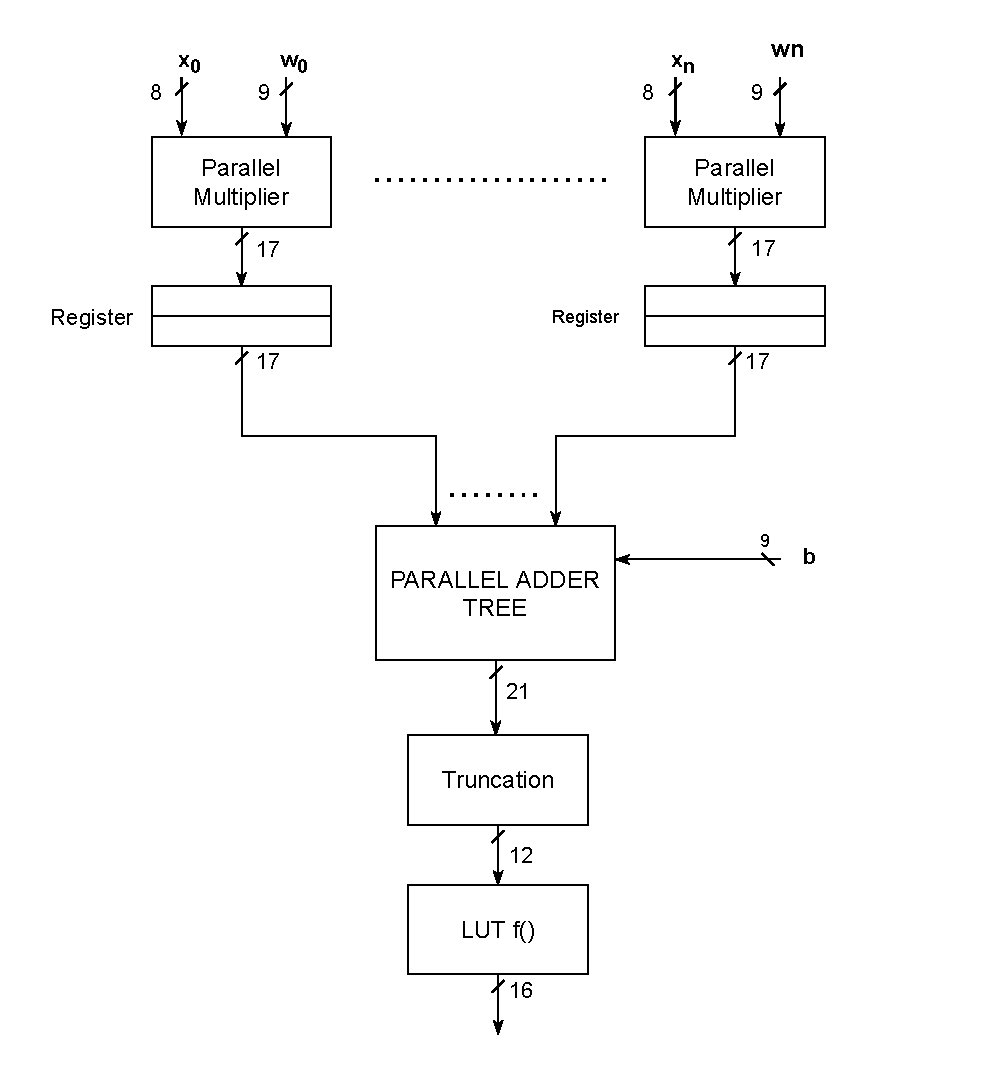
\includegraphics[width=12cm]{img/architecture_general_schema.pdf}
	\caption{General Schema}
\end{figure}

\subsection{Multiplication Circuit Architecture}
The Multiplication Circuit, as said before, will be implemented through a Parallel Multiplier. The inputs $b_{i}$ and $w_{i}$ are composed respectively by $b_{x} = 8$ bits and $b_{w} = 9$ bits. In order to compute the multiplication in the correct way, the inputs need to be translated in the \textbf{unsigned form} and then is possible to perform the multiplication with the parallel multiplier.
In the following image is presented the general schema of the Parallel Multiplier:
\begin{figure}[H]
	\centering
	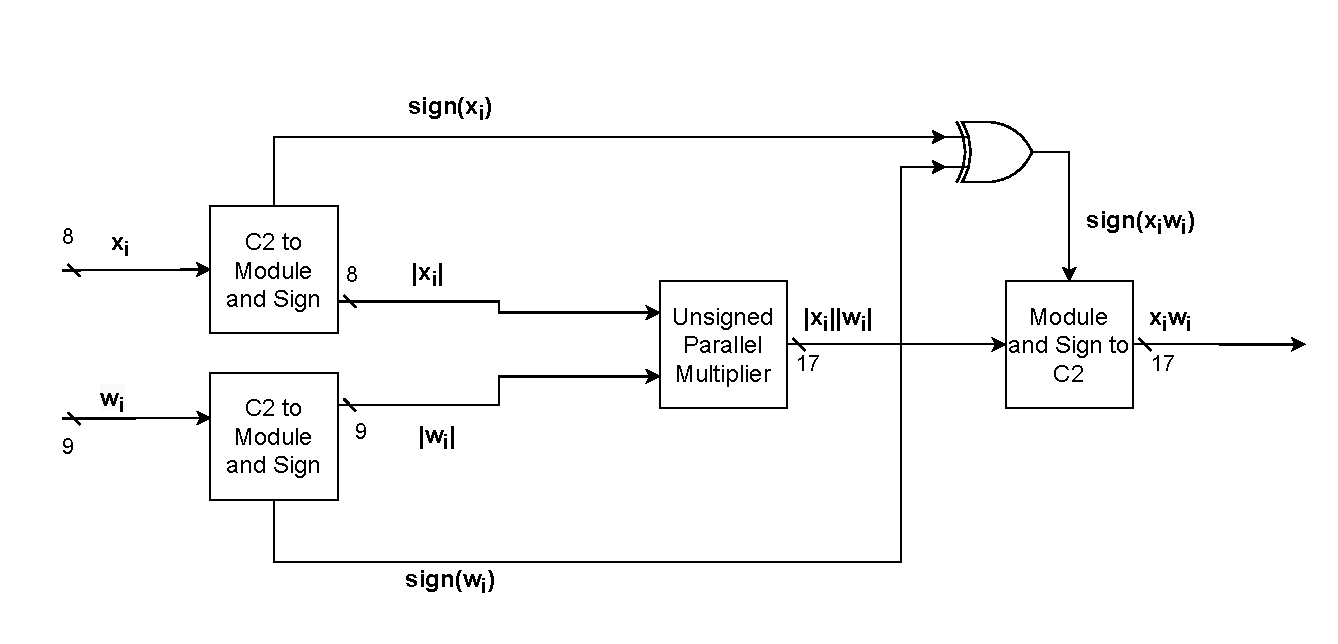
\includegraphics[width=\textwidth]{img/architecture_general_parallel_multiplier.pdf}
	\caption{Parallel Multiplier Architecture}
\end{figure}
Notice that the \textbf{sign} of the result will be computed by a simple \textit{XOR} operation between the inputs signs. 
The \textbf{Unsigned Parallel Multiplier} architecture is the following:
\begin{figure}[H]
	\centering
	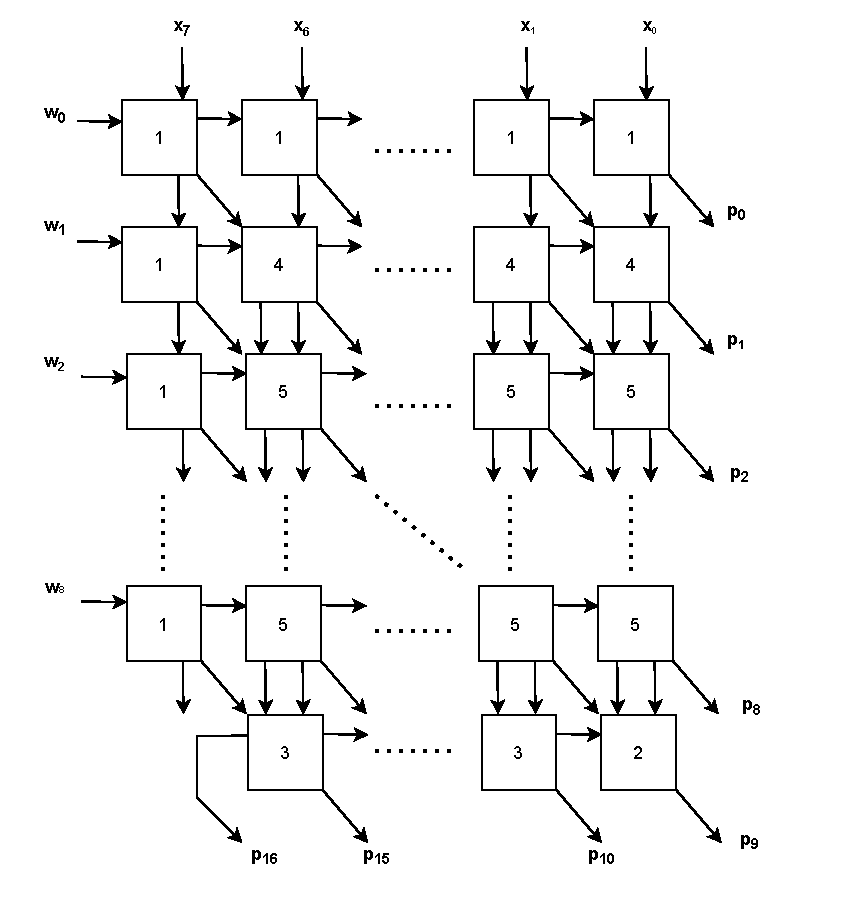
\includegraphics[width=13cm]{img/architecture_parallel_multiplier.pdf}
	\caption{Unsigned Parallel Multiplier Architecture}
\end{figure}
Each logic block is translated with a related logic block:
\begin{figure}[H]
	\centering
	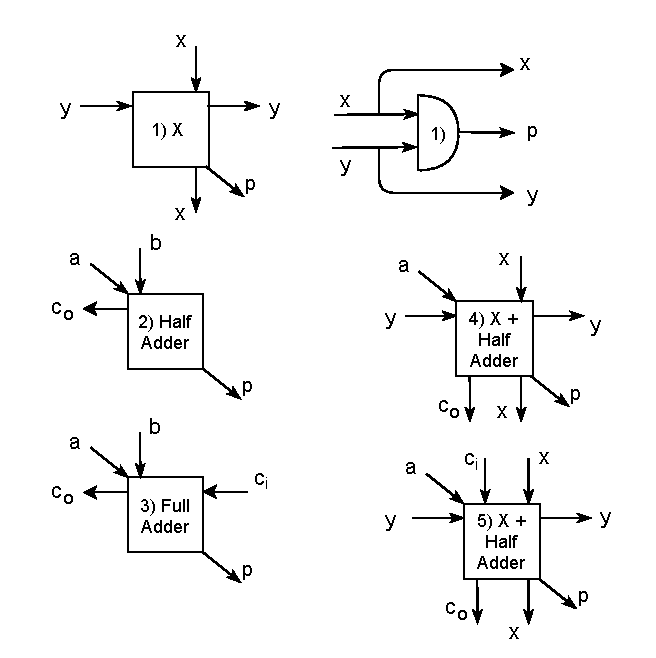
\includegraphics[width=0.7\textwidth]{img/architecture_parallel_multiplier_meaning.pdf}
	\caption{Unsigned Parallel Multiplier Architecture}
\end{figure}
\subsection{Adder Circuit Architecture}
In order to compute the equation (1.1) different sums need to be computed. The building block of this part will be the \textbf{Parallel Adder with Pipeline}: as said before, by adding some registers in between the Carry chains, the critical path impact can be reduced. Furthermore, by exploiting the parallel architecture, a single sum can be computed in a single clock cycle. In the next figure will be presented the Parallel Adder:
 \begin{figure}[H]
 	\centering
 	\makebox[\textwidth][c]{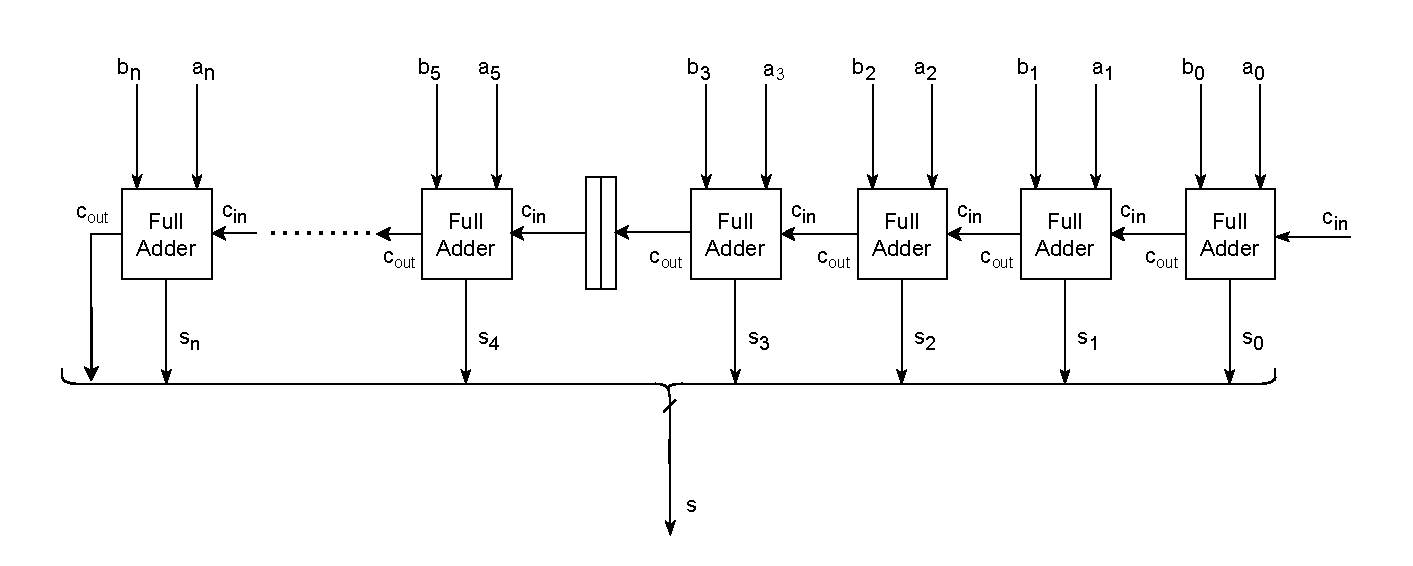
\includegraphics[width=1.5\textwidth]{img/architecture_full_adder_with_pipeline.pdf}}%
 	\caption{Parallel Adder Architecture}
 \end{figure}
In order to obtain an output, after an input drive, there is a need to wait $\floor*{\frac{N}{N_{pipeline}}}$ clock cycles, where $N$ represent the number of bits of $a$ or $b$ and $N_{pipeline}$ represent the maximum number of consecutive FA without a register in between.\\
To implement the whole sum of 11 terms, \textbf{in order to decrease the number of cycles needed} to compute the whole sum and to reduce the number of bits needed, a tree approach has been chosen. The schema of the tree parallel adder is the following:
\begin{figure}[H]
	\centering
	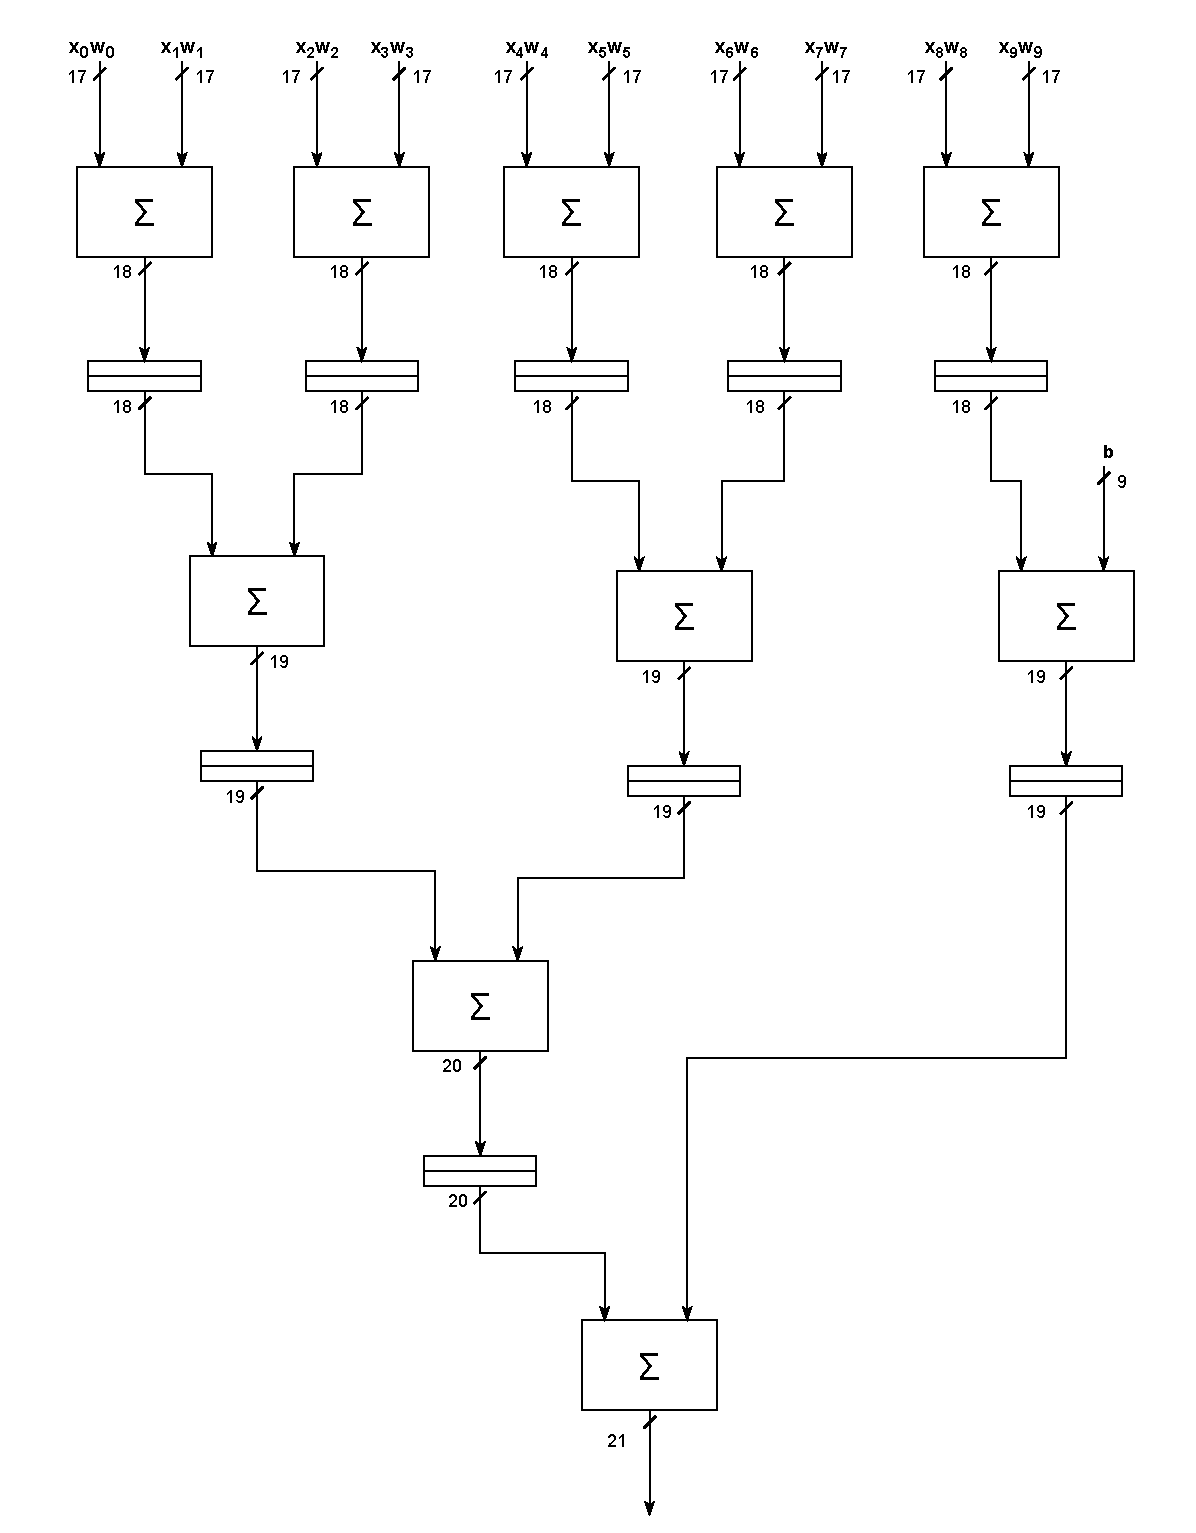
\includegraphics[width=\textwidth]{img/architecture_adder_tree.pdf}
	\caption{Parallel Multiplier Architecture}
\end{figure}

\textbf{Note some extension or left shifts (i.e. for b) were not represented.}\\
Some register has been put in between the sum to limit the critical path impact on the performances and clock period limit. 
To obtain a good output after an input drive there is a need to sum to 3 (the maximum number of consecutive register in the previous architecture) each Ripple Carry Adder contribution in terms of number of clock as seen before.

\subsection{Activation Function Circuit Architecture}
At the end of the computation of the latter phase the output is composed by $21$ bits. The computation of the sigmoid function will be done through a \textbf{Look-Up-Table}, which will need \textbf{$2^{21} = $ 2097152 entries} of different outputs with $16$ bits. In order to reduce the size of the Look-Up-Table a truncation is needed: from $21$ bits to $12$ bits. In this case the Look-Up Table will be composed by \textbf{$2^{12} = $ 4096 entries}, but, by exploiting the \textbf{odd symmetry} of the sigmoid, only \textbf{$4096/2 = $ 2048 entries} are needed.
\begin{figure}[H]
	\centering
	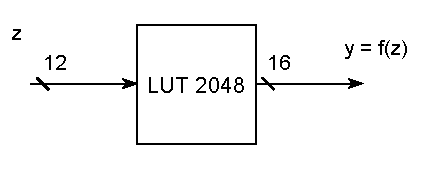
\includegraphics[width=0.6\textwidth]{img/architecture_lut_optimized.pdf}
	\caption{Look-Up Table Architecture}
\end{figure}

All things considered, by performing the calculation showed before, there is a need of 26 \textbf{clock cycles} to obtain a correct output after driving an input.
 
\section{VHDL CODE}
In this chapter will be presented the main modules that compose the architecture of the \textbf{Perceptron with sigmoid activation function}.
\subsection{Modules List}
As presented in the last chapter, I have followed a similar approach for creating the architecture. The following modules were created:

\begin{itemize}
	\item Perceptron
	\begin{itemize}
		\item Parallel$\_$Multiplier
  		\begin{itemize}
  			\item Unsigned Parallel Multiplier
  			\begin{itemize}
	  			\item Full Adder
	  			\item Half Adder
  			\end{itemize}
		\end{itemize}
	\end{itemize}
	\begin{itemize}
		\item Tree$\_$Adder
		\begin{itemize}
			\item Ripple$\_$Carry$\_$Adder$\_$Pipelined
			\begin{itemize}
				\item DFF
				\item Full Adder
			\end{itemize} 
		\end{itemize} 
	\end{itemize}
	\begin{itemize}
		\item Sigmoid$\_$Lut$\_$2048
	\end{itemize}
\end{itemize}

A \textbf{bottom-up strategy} was followed in order to build the architecture: starting from the some modules that will made up the architecture and after finishing each of them some testbenches were written in order to test each building block of the \textbf{Perceptron} (See next chapter for details).
\subsection{Perceptron}
The main hardware description of the architecture. In order to not show too much lines of code only the entity definition of this module will be shown.
\begin{lstlisting}[language=VHDL]
	library IEEE;
	use IEEE.std_logic_1164.all;
	use IEEE.numeric_std.all;
	entity Perceptron is
	port(
	
	-- x_1 to x_10 inputs of the perceptron with 8 bits
	x_1: in std_logic_vector(7 downto 0);
	x_2: in std_logic_vector(7 downto 0);
	x_3: in std_logic_vector(7 downto 0);
	x_4: in std_logic_vector(7 downto 0);
	x_5: in std_logic_vector(7 downto 0);
	x_6: in std_logic_vector(7 downto 0);
	x_7: in std_logic_vector(7 downto 0);
	x_8: in std_logic_vector(7 downto 0);
	x_9: in std_logic_vector(7 downto 0);
	x_10: in std_logic_vector(7 downto 0);
	
	-- w_1 to w_10 inputs of the perceptron with 9 bits
	w_1: in std_logic_vector(8 downto 0);
	w_2: in std_logic_vector(8 downto 0);
	w_3: in std_logic_vector(8 downto 0);
	w_4: in std_logic_vector(8 downto 0);
	w_5: in std_logic_vector(8 downto 0);
	w_6: in std_logic_vector(8 downto 0);
	w_7: in std_logic_vector(8 downto 0);
	w_8: in std_logic_vector(8 downto 0);
	w_9: in std_logic_vector(8 downto 0);
	w_10: in std_logic_vector(8 downto 0);
	
	-- b input of the perceptron with 9 bits
	b: in std_logic_vector(8 downto 0);
	
	clk: in std_logic;
	rst: in std_logic;
	
	-- output of the perceptron 16 bits
	f_z: out std_logic_vector(15 downto 0)
	);
	end Perceptron;
\end{lstlisting}

In the rest of this modules are instantiated and linked the various submodule that made up the \textbf{Perceptron} module.

\subsection{Parallel Multiplier}
\begin{lstlisting}[language=VHDL]
	library IEEE;
	use IEEE.std_logic_1164.all;
	use ieee.numeric_std.all;
	
	
	entity Parallel_Multiplier is
	generic (
	Nbit_a : positive; 
	Nbit_b: positive
	);
	port(
	a_p_signed: in std_logic_vector(Nbit_a - 1 downto 0);
	b_p_signed: in std_logic_vector(Nbit_b - 1 downto 0);
	p_signed: out std_logic_vector(Nbit_a + Nbit_b - 1 downto 0)
	);
	end entity Parallel_Multiplier;
	
	architecture rtl of Parallel_Multiplier is
	
	-- Building blocks of the Parallel Multiplier
	component Unsigned_Parallel_Multiplier
	generic(
	Nbit_a : positive;
	Nbit_b : positive
	);
	port(
	a_p: in  std_logic_vector(Nbit_a - 1 downto 0);
	b_p : in  std_logic_vector(Nbit_b - 1 downto 0);
	p   : out std_logic_vector(Nbit_a + Nbit_b - 1 downto 0)
	);
	end component Unsigned_Parallel_Multiplier;
	
	
	-- Unsigned component (will work for the unsigned parallel multiplier
	signal p_unsigned: std_logic_vector(Nbit_a + Nbit_b - 1 downto 0);
	signal a_p_unsigned: std_logic_vector(Nbit_a - 1 downto 0);
	signal b_p_unsigned: std_logic_vector(Nbit_b - 1 downto 0);
	
	-- will carry the sign bit for the signed rapresentation of the inputs
	signal a_sign: std_logic;
	signal b_sign: std_logic;
	
	begin
	
	-- Compute the unsigned representation from the signed one
	a_p_unsigned <= std_logic_vector(abs(signed(a_p_signed)));
	b_p_unsigned <= std_logic_vector(abs(signed(b_p_signed)));
	
	-- 2's complement rapresentation, the result sign uis computed through the xor op. between a and b
	p_signed <= std_logic_vector(unsigned(not(p_unsigned)) + 1) when (((a_sign xor b_sign) = '1')) else p_unsigned;
	
	-- Getting of the sign from a and b (the MSB of the C2 representation)
	a_sign <= a_p_signed(Nbit_a - 1);
	b_sign <= b_p_signed(Nbit_b - 1);
	
	unsigned_parallel_mul: Unsigned_Parallel_Multiplier
	generic map(
	Nbit_a => Nbit_a,
	Nbit_b => Nbit_b
	)
	port map(
	a_p =>  a_p_unsigned,
	b_p =>  b_p_unsigned,
	p   => p_unsigned
	);
	
	end architecture rtl; 
\end{lstlisting}

\subsection{Unsigned Parallel Multiplier}
\begin{lstlisting}[language=VHDL]
	library IEEE;
	use IEEE.std_logic_1164.all;
	
	entity Unsigned_Parallel_Multiplier is
	generic (
	Nbit_a : positive; 
	Nbit_b: positive
	);
	port(
	-- Unsigned representation of inputs
	a_p: in std_logic_vector(Nbit_a - 1 downto 0);
	b_p: in std_logic_vector(Nbit_b - 1 downto 0);
	
	-- p = a_p * b_p
	p: out std_logic_vector(Nbit_a + Nbit_b - 1 downto 0)
	);
	end entity Unsigned_Parallel_Multiplier;
	
	architecture rtl of Unsigned_Parallel_Multiplier is
	-- Building blocks of the Unsigned Parallel Multiplier
	component FULL_ADDER is
	port
	(
	a    : IN std_logic ;
	b    : IN std_logic ;
	cin  : IN std_logic ;
	s    : OUT std_logic ;
	cout : OUT std_logic 
	);
	end component;
	
	component HALF_ADDER is
	port
	(
	a    : IN std_logic ;
	b    : IN std_logic ;
	s    : OUT std_logic ;
	cout : OUT std_logic 
	);
	end component;
	
	-- Will hold the carry signals among the whole architecture
	signal carry_signal: std_logic_vector((Nbit_a - 1)*(Nbit_b - 1) - 1 downto 0);
	signal last_carry_signal: std_logic_vector((Nbit_b - 1) downto 0);
	
	-- Will hold the sum result of the FA and HA among the whole architecture
	signal sum_signal: std_logic_vector((Nbit_a - 1)*(Nbit_b - 2) - 1 downto 0);  
	
	-- will hold the precomputed values for the inputs a and b of the various Half Adder and Full Adder
	signal a_multiplier: std_logic_vector(Nbit_a + Nbit_b - 2 downto 0);
	signal b_multiplier: std_logic_vector((Nbit_a - 1)*(Nbit_b - 1) - 1 downto 0);
	
	begin
	
	-- First bit of the result
	p(0) <= (a_p(0) and b_p(0));
	
	
	-- Computation of the various inputs of each HA and FA
	d_process: process(a_p, b_p)
	begin
	
	for j in 1 to Nbit_b loop
	a_multiplier(j - 1) <= (a_p(0) and b_p(Nbit_b - j));
	end loop;
	
	for i in 2 to Nbit_a loop
	a_multiplier(Nbit_b + i - 2) <= (a_p(i - 1) and b_p(Nbit_b - 1));
	end loop;
	
	for i in 1 to Nbit_a-1 loop
	for j in 1 to Nbit_b - 1 loop
	b_multiplier((i-1)*(Nbit_b -1) + j - 1) <= (a_p(i) and b_p(Nbit_b - j - 1));
	end loop;
	end loop;
	end process d_process;
	
	
	-- Architecture will follow schema of the Parallel Multiplier
	-- Row index i
	GEN_a: for i in 1 to Nbit_a generate
	-- Column index j
	GEN_b: for j in 1 to Nbit_b - 1 generate 
	FIRST_ROW: if i=1 generate
	-- In the first Row only HA
	LEFT: if j < Nbit_b -1 generate
	ROW1_LEFT: HALF_ADDER
	port map
	(
	a    => a_multiplier(j - 1), 
	b    => b_multiplier(j - 1), 
	s    => sum_signal(j - 1), 
	cout => carry_signal(j - 1) 
	);
	end generate LEFT;
	RIGHT: if j = Nbit_b - 1 generate
	ROW1_RIGHT: HALF_ADDER
	port map
	(
	a    => a_multiplier(j - 1), 
	b    => b_multiplier(j - 1), 
	s    => p(1), -- Result bit 
	cout => carry_signal(j - 1) 
	);
	end generate RIGHT; 
	end generate FIRST_ROW;
	
	
	INTERNAL_ROW: if i > 1 and i < Nbit_a generate
	-- Internal Rows only FA
	LEFT: if j = 1 generate 
	ROW_INT_LEFT: FULL_ADDER
	port map
	(
	a => a_multiplier(Nbit_b + i - 2),  
	b => b_multiplier((i-1)*(Nbit_b -1) + j - 1), 
	cin => carry_signal((i-2)*(Nbit_b - 1) + (j-1)), 
	s => sum_signal((i-1)*(Nbit_b - 2) + (j-1)), 
	cout => carry_signal((i-1)*(Nbit_b - 1) + (j-1)) 
	);
	end generate LEFT;
	CENTER: if j > 1 and j < Nbit_b - 1 generate
	ROW_INT_CENTER: FULL_ADDER
	port map
	(
	a => sum_signal((i-2)*(Nbit_b - 2) + (j-2)), 
	b =>  b_multiplier((i-1)*(Nbit_b -1) + j - 1), 
	cin => carry_signal((i-2)*(Nbit_b - 1) + (j-1)),
	s => sum_signal((i-1)*(Nbit_b - 2) + (j-1)),
	cout => carry_signal((i-1)*(Nbit_b - 1) + (j-1))
	);
	end generate CENTER;
	RIGHT: if j = Nbit_b - 1 generate
	ROW_INT_RIGHT: FULL_ADDER
	port map
	(
	a => sum_signal((i-2)*(Nbit_b - 2) + (j-2)), 
	b => b_multiplier((i-1)*(Nbit_b -1) + j - 1), 
	cin => carry_signal((i-2)*(Nbit_b - 1) + (j-1)), 
	s => p(i), -- Result bit
	cout => carry_signal((i-1)*(Nbit_b - 1) + (j-1)) 
	);
	end generate RIGHT;
	end generate INTERNAL_ROW;
	
	
	LAST_ROW: if i = Nbit_a generate
	-- Last row FA and an HA on the rightmost block
	LEFT: if j = 1 generate 
	ROW_INT_LEFT: FULL_ADDER
	port map
	(
	a => a_multiplier(Nbit_b + i - 2), 
	b => carry_signal((i-2)*(Nbit_b - 1) + (j-1)), 
	cin => last_carry_signal(Nbit_b - j), 
	s => p((Nbit_a) + (Nbit_b) - 1 - j), -- Result bit
	cout => p((Nbit_a) + (Nbit_b) -1) -- Result bit
	);
	end generate LEFT;
	CENTER: if j > 1 and j < Nbit_b - 1 generate
	ROW_INT_CENTER: FULL_ADDER
	port map
	(
	a => sum_signal((i-2)*(Nbit_b - 2) + (j-2)), 
	b =>  carry_signal((i-2)*(Nbit_b - 1) + (j-1)), 
	cin => last_carry_signal(Nbit_b - j), 
	s =>  p((Nbit_a) + (Nbit_b) - 1 - j), -- Result bit
	cout =>last_carry_signal(Nbit_b - j + 1) 
	);
	end generate CENTER;
	RIGHT: if j = Nbit_b - 1 generate
	ROW_INT_RIGHT: HALF_ADDER
	port map
	(
	a => sum_signal((i-2)*(Nbit_b - 2) + (j-2)),
	b => carry_signal((i-2)*(Nbit_b - 1) + (j-1)), 
	s => p((Nbit_a) + (Nbit_b) -1 - j), -- Result bit
	cout =>last_carry_signal(Nbit_b - j + 1)
	);
	end generate RIGHT;
	end generate LAST_ROW;
	end generate GEN_b;
	end generate GEN_a;
	end architecture rtl; 
\end{lstlisting}

\subsection{Tree Adder}
\begin{lstlisting}[language=VHDL]
library IEEE;
use IEEE.std_logic_1164.all;

entity Tree_Adder is
port(
-- Inputs: result of the multiplication of xi*wi
in_1: in std_logic_vector(16 downto 0);
in_2: in std_logic_vector(16 downto 0);
in_3: in std_logic_vector(16 downto 0);
in_4: in std_logic_vector(16 downto 0);
in_5: in std_logic_vector(16 downto 0);
in_6: in std_logic_vector(16 downto 0);
in_7: in std_logic_vector(16 downto 0);
in_8: in std_logic_vector(16 downto 0);
in_9: in std_logic_vector(16 downto 0);
in_10: in std_logic_vector(16 downto 0);

-- Bias input
b: in std_logic_vector(8 downto 0);
clk: in std_logic;
rst: in std_logic;

-- Output
z: out std_logic_vector(20 downto 0)
);
end Tree_Adder;

\end{lstlisting}

\subsubsection{Ripple Carry Adder Pipelined}
\begin{lstlisting}[language=VHDL]
library IEEE;
use IEEE.std_logic_1164.all;

-- Realize a Ripple Carry Adder in a structural way

entity Ripple_Carry_Adder_Pipelined is
generic (Nbit: positive);
port(
-- Inputs
a_r: in std_logic_vector(Nbit-2 downto 0);
b_r: in std_logic_vector(Nbit-2 downto 0);
cin_r: in std_logic;
cout_r: out std_logic;

-- Will store the result of a_r+b_r
s_r: out std_logic_vector(Nbit-1 downto 0);
clk: in std_logic;
rst: in std_logic
);
end Ripple_Carry_Adder_Pipelined;

architecture rtl of Ripple_Carry_Adder_Pipelined is 
-- Building blocks of the Ripple Carry Adder Pipelined 
component FULL_ADDER
port(
a: in std_logic;
b: in std_logic;
cin: in std_logic;
s: out std_logic;
cout: out std_logic
);
end component FULL_ADDER;

-- Need of a register to obtain the pipelined version
component DFF
port(
d_dff      : in  std_logic;
clk_dff    : in  std_logic;
resetn_dff : in  std_logic;
q_dff      : out std_logic
);
end component DFF;

signal carry_signal: std_logic_vector(Nbit-1 downto 1);
signal dff_signal: std_logic_vector(Nbit-1 downto 0) := (others => '0');

begin
-- Implemented in a structured way in a similar fashion as seen in the Lab lessions
GEN: for i in 1 to Nbit generate
FIRST: if i=1 generate
-- First FA
FFI: FULL_ADDER port map (a_r(0), b_r(0), cin_r, s_r(0), carry_signal(1));
end generate FIRST;
INTERNAL: if i > 1 and i < Nbit generate
-- Need of Register detection
PIPE: if (i mod 3 = 0) generate
DFF_I: DFF
port map(
d_dff      => carry_signal(i-1),
clk_dff    => clk,
resetn_dff => rst,
q_dff      => dff_signal(i-1)
);
FFI: FULL_ADDER port map (a_r(i-1), b_r(i-1), dff_signal(i-1), s_r(i-1), carry_signal(i));
end generate PIPE;
-- No need of a register
NOT_PIPE: if (i mod 3 /= 0) generate
FFI: FULL_ADDER port map (a_r(i-1), b_r(i-1), carry_signal(i-1), s_r(i-1), carry_signal(i));
end generate NOT_PIPE;           
end generate INTERNAL;

-- Implicit extension (the inputs have Nbit-2 bits, the output has Nbit-1 bits and there
-- are Nbit-1 FA so the last bit is replicated in order to make the extension in the 
-- correct way in C2 representation)

LAST: if i=Nbit generate
FFI: FULL_ADDER port map (a_r(Nbit-2), b_r(Nbit-2), carry_signal(Nbit-1), s_r(Nbit-1), cout_r);
end generate LAST;
end generate GEN;
end rtl;

\end{lstlisting}

\subsection{LUT}
\begin{lstlisting}[language=VHDL]
library IEEE;
use IEEE.std_logic_1164.all;
use IEEE.numeric_std.all;

entity sigmoid_lut_2048 is
port (
address : in  std_logic_vector(10 downto 0);
dds_out : out std_logic_vector(15 downto 0) 
);
end sigmoid_lut_2048;


-- Output between [-11; +11], rapresented with fixed point
-- Need for 1 bit for integer, last 15 bit for float rapresentation
-- Reach the LSB method
-- 
-- LSB(in) = (11)/(2^11 - 1) = 0.00537371763556424035173424523693
-- LSB(out) = (1)/(2^15 - 1) = 3.0518509475997192297128208258309e-5
-- inputs -> [-11, +11] 
-- outputs -> [0, 1]
-- Q(f(x)) = round(f(x)/LSB(out))*LSB(out)
-- 
--
-- What to store in the lut? round(f(x)/LSB(out)) for x in [0; 2047]*LSB(in)

architecture rtl of sigmoid_lut_2048 is
type LUT_t is array (natural range 0 to 2047) of integer;
constant LUT: LUT_t := (
0 => 16384,
1 => 16428,
...
2046 => 32766,
2047 => 32766
);

begin
dds_out <= std_logic_vector(TO_SIGNED(LUT(TO_INTEGER(unsigned(address))),16));
end rtl;	
\end{lstlisting}

\subsubsection{Lut generation code}
\begin{lstlisting}[language=Python]
	"""
	LSB(out) = (1)/(2^15 - 1) = 3.0518509475997192297128208258309e-5
	LSB(in) = (11)/(2^11 - 1) = 0.00537371763556424035173424523693
	
	What to store in the lut? round(f(x)/LSB(out)) for x in [0; 2047]*LSB(in)
	"""
	
	import math
	
	#Calculate lsb of x (16 bits) and f(x) (12 bits)
	lsb_out = (1)/(2**15 - 1)
	lsb_in = (11)/(2**11 - 1)
	result = ""
	
	
	for x in range(0, 2048):
		f_x = (1)/(1 + math.exp(-(x*lsb_in)))
		lut = round(f_x/lsb_out)
		
		#Generate lut entries for every x
		result += str(x) + " => " + str(lut) + ",\n"
	
	print(result)
	
\end{lstlisting}
\section{Test Plan}
In order to verify the correctness of the system the following tests were made:
\begin{enumerate}
	\item \textbf{Unit Tests}: following the \textbf{bottom-up} strategy, each sub-module (Parallel Multiplier, Ripple Carry Adder Pipelined...), after completing the implementation, has a dedicated testbench in order to check the correctness of the single sub-module in isolation. Considering the fact that this test are \textbf{trivial} (just checking if the sum or the product of some numbers is correct) the single modules were not separately implemented in python. So this part will not be showed in this documentation.
	\item \textbf{System Estimation Test}: in this phase, some testbenches were written with particular inputs. The aim of this test is only to check if the result will resemble the sigmoid curve by varying the inputs in time in an increasing way.
	\item \textbf{System Aimed Test}: after checking that the system is \textit{likely} correct by the latter test, through a python script will be made a test with different inputs in the range considered and check, with an additional testbench, if the outputs are equal.
\end{enumerate}
\subsection{System Estimation Test}
Even before checking the correctness of the output of the system by a given input, three "estimation tests" were made. The aim of these tests is just to obtain a sigmoid curve by setting each $x_{i}$ and $w_{i}$ and varying the bias $b$ in the range of $[-1; +1]$.
\subsubsection{Estimation Test 1}
In this case we have the \textbf{following inputs}:
\begin{equation}
	x_{1} \dots x_{10} = 0, w_{1} \dots w_{10} = 0
\end{equation}
The bias b will vary in the whole range of $[-1, +1]$. Just to remind the sigmoid function curve, we \textbf{expect to obtain a curve with an odd symmetry and a "linear" behaviour}, due to the fact that we are considering the values near zero of the curve:
\begin{figure}[H]
	\centering
	\caption{Sigmoid Function Plot}
	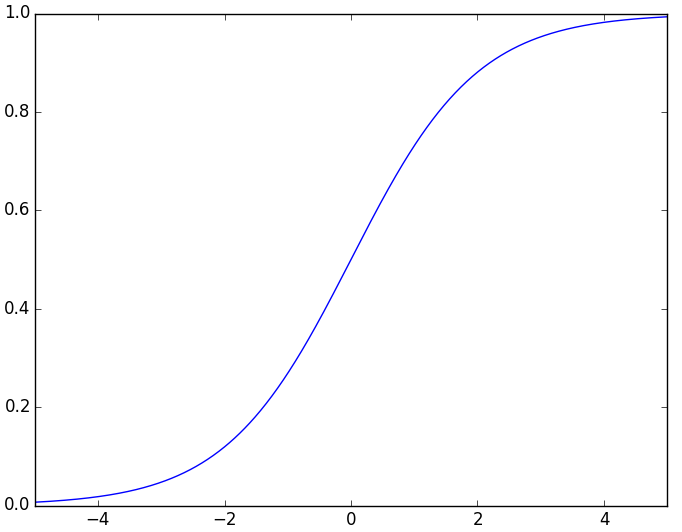
\includegraphics[width=8cm]{img/sigmoid.png}
\end{figure}
The output of the system is the following:
\begin{figure}[H]
	\centering
	\caption{Output of the System 1}
	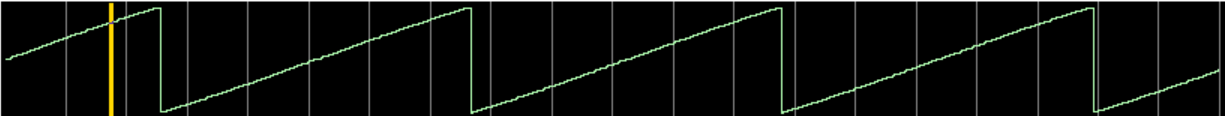
\includegraphics[width=\textwidth]{img/est_test_1.png}
\end{figure}
There are different replication of the system due to the fact that the bias b will "turn back" when he will get to his maximum. We can state that, by comparing the two figures, the \textbf{first estimation test is passed}. 
\subsubsection{Estimation Test 2}
\begin{equation}
	x_{1} \dots x_{10} \approx 1, w_{1} \dots w_{10} \approx 1
\end{equation}
The bias b will vary in the whole range of $[-1, +1]$. \textbf{We expect to obtain a likely flat curve with some "high values"} due to the fact that the summation of the ten product is 10 and the sigmoid at that value tends to 1.
\begin{figure}[H]
	\centering
	\caption{Output of the System 2}
	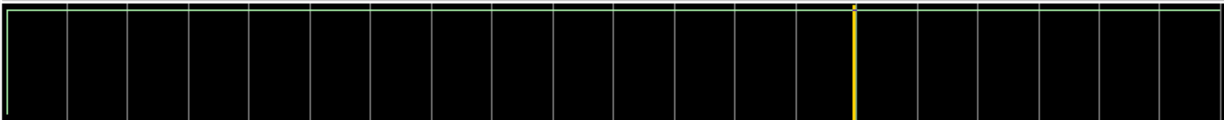
\includegraphics[width=\textwidth]{img/est_test_2.png}
\end{figure}
The output of the system is similar to a flat curve. We can state that, by comparing the system output with what we expected, the \textbf{second estimation test is passed}.
\subsubsection{Estimation Test 3}
\begin{equation}
	x_{1} \dots x_{10} \approx -1, w_{1} \dots w_{10} \approx 1
\end{equation}
The bias b will vary in the whole range of $[-1, +1]$.\textbf{ We expect to obtain a likely flat curve with some "low values"} due to the fact that the summation of the ten product is -10.
\begin{figure}[H]
	\centering
	\caption{Output of the System 3}
	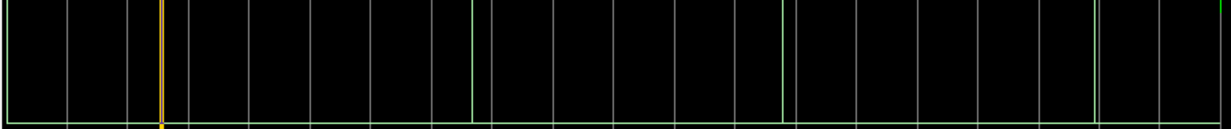
\includegraphics[width=\textwidth]{img/est_test_3.png}
\end{figure}
The curve is flat with low values but we can notice some \textit{noise}. This is due to the fact that to obtain a proper output some clock cycles are needed: this will lead to obtain intermediate results that are not good. But we can state that, by comparing the system output with what we expected, the \textbf{third estimation test is passed}.
\subsection{System Aimed Test}
At this point will be carried out some tests with the same inputs using the \textbf{Perceptron} architecture realized at this point and a \textit{python script} which will simulate the desired behaviour of the \textbf{Perceptron}. The latter is described through the following script:

\begin{lstlisting}[language=python]
import math

def get_outputs(i, x, w, b):
	print(f"################### TEST #{i} ###################")
	print(f"X: {x}")
	print(f"W: {w}")
	print(f"b: {b}")
	
	sum = summation(x, w, b)
	print(f"Sum result:\t\t\t\t {sum}")
	
	f_z = sigmoid_output(sum)
	print(f"Sigmoid output:\t\t\t {f_z}")
	
	#the sum with 12 bits
	sum_in_circuit = round(sum/lsb_in)
	print(f"Sum value quantized:\t {sum_in_circuit}")

	f_z_in_circuit = round(f_z/lsb_out)
	print(f"Output value quantized:\t {f_z_in_circuit}")

def summation(x, w, b):
	sum = 0
	for i in range(0, 10):
		sum += x[i]*w[i]
	sum += b
	return sum

def sigmoid_output(s):
	res = (1)/(1 + math.exp(-s))
	return res

lsb_out = (1)/(2**15 - 1)
lsb_in = (32)/(2**11 - 1)
#Test #1
x = [-1,-1,-1,-1,-1,-1,-1,-1,-1,-1]
w = [1,1,1,1,1,1,1,1,1,1]
b = 0
get_outputs(1, x, w, b)
...
#Other tests
...
\end{lstlisting}

By running the python script the following output has been displayed in the console:

\begin{lstlisting}
################### TEST #1 ###################
X: [-1, -1, -1, -1, -1, -1, -1, -1, -1, -1]
W: [1, 1, 1, 1, 1, 1, 1, 1, 1, 1]
b: 0
Sum result:				 -10
Sigmoid output:			 4.5397868702434395e-05
Sum value quantized:	 -640
Output value quantized:	 1
################### TEST #2 ###################
X: [-0.75, -0.75, -0.75, -0.75, -0.75, -0.75, -0.75, -0.75, -0.75, -0.75]
W: [1, 1, 1, 1, 1, 1, 1, 1, 1, 1]
b: 0
Sum result:				 -7.5
Sigmoid output:			 0.0005527786369235996
Sum value quantized:	 -480
Output value quantized:	 18
################### TEST #3 ###################
X: [-0.5, -0.5, -0.5, -0.5, -0.5, -0.5, -0.5, -0.5, -0.5, -0.5]
W: [1, 1, 1, 1, 1, 1, 1, 1, 1, 1]
b: 0
Sum result:				 -5.0
Sigmoid output:			 0.0066928509242848554
Sum value quantized:	 -320
Output value quantized:	 219
################### TEST #4 ###################
X: [-0.5, -0.5, -0.5, -0.5, -0.5, -0.5, -0.5, -0.5, -0.5, -0.5]
W: [0.5, 0.5, 0.5, 0.5, 0.5, 0.5, 0.5, 0.5, 0.5, 0.5]
b: 0
Sum result:				 -2.5
Sigmoid output:			 0.07585818002124355
Sum value quantized:	 -160
Output value quantized:	 2486
################### TEST #5 ###################
X: [-0.5, -0.5, -0.5, -0.5, -0.5, -0.5, -0.5, -0.5, -0.5, -0.5]
W: [0, 0, 0, 0, 0, 0, 0, 0, 0, 0]
b: 0
Sum result:				 0.0
Sigmoid output:			 0.5
Sum value quantized:	 0
Output value quantized:	 16384
################### TEST #6 ###################
X: [-0.5, -0.5, -0.5, -0.5, -0.5, -0.5, -0.5, -0.5, -0.5, -0.5]
W: [-0.5, -0.5, -0.5, -0.5, -0.5, -0.5, -0.5, -0.5, -0.5, -0.5]
b: 0
Sum result:				 2.5
Sigmoid output:			 0.9241418199787566
Sum value quantized:	 160
Output value quantized:	 30281
################### TEST #7 ###################
X: [0.5, 0.5, 0.5, 0.5, 0.5, 0.5, 0.5, 0.5, 0.5, 0.5]
W: [1, 1, 1, 1, 1, 1, 1, 1, 1, 1]
b: 0
Sum result:				 5.0
Sigmoid output:			 0.9933071490757153
Sum value quantized:	 320
Output value quantized:	 32548
################### TEST #8 ###################
X: [0.75, 0.75, 0.75, 0.75, 0.75, 0.75, 0.75, 0.75, 0.75, 0.75]
W: [1, 1, 1, 1, 1, 1, 1, 1, 1, 1]
b: 0
Sum result:				 7.5
Sigmoid output:			 0.9994472213630764
Sum value quantized:	 480
Output value quantized:	 32749
################### TEST #9 ###################
X: [1, 1, 1, 1, 1, 1, 1, 1, 1, 1]
W: [1, 1, 1, 1, 1, 1, 1, 1, 1, 1]
b: 0
Sum result:				 10
Sigmoid output:			 0.9999546021312976
Sum value quantized:	 640
Output value quantized:	 32766
################### TEST #10 ###################
X: [1, 1, 1, 1, 1, 1, 1, 1, 1, 1]
W: [1, 1, 1, 1, 1, 1, 1, 1, 1, 1]
b: 1
Sum result:				 11
Sigmoid output:			 0.999983298578152
Sum value quantized:	 704
Output value quantized:	 32766
################### TEST #11 ###################
X: [-1, -1, -1, -1, -1, -1, -1, -1, -1, -1]
W: [1, 1, 1, 1, 1, 1, 1, 1, 1, 1]
b: -1
Sum result:				 -11
Sigmoid output:			 1.670142184809518e-05
Sum value quantized:	 -704
Output value quantized:	 1
\end{lstlisting}

By running a new testbench with \textbf{likely} the same inputs the following results were displayed in \textbf{Modelsim}:
\begin{figure}[H]
	\centering
	\caption{Output of the System 3}
	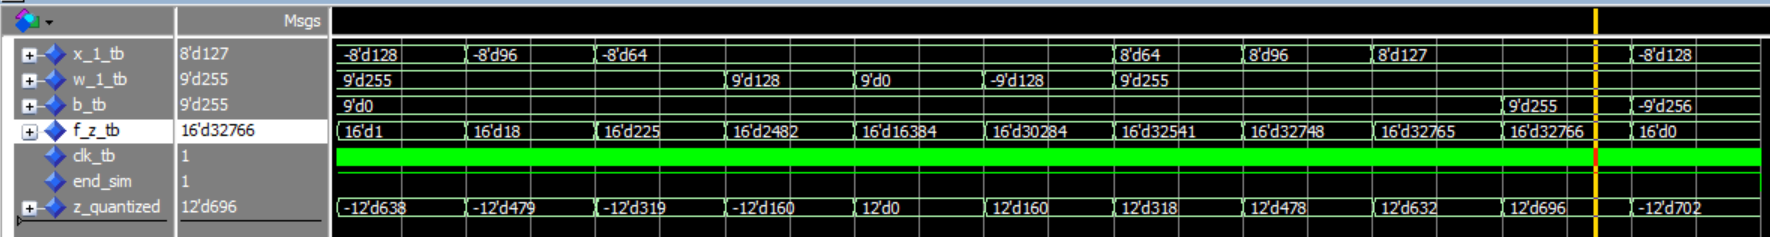
\includegraphics[width=\textwidth]{img/aimed_test.png}
\end{figure}

A comparison with the outputs can be seen in the following table:
\begingroup
\setlength{\tabcolsep}{10pt} % Default value: 6pt
\renewcommand{\arraystretch}{2} % Default
\begin{center}
	\begin{tabular}{|p{2cm}||p{2.4cm}|p{2.4cm}|p{2.4cm}|p{2.4cm}|}
		\hline
		\multirow{2}{*}{\textbf{Test}}  & \multicolumn{2}{|p{3cm}|}{\textbf{Python Script}} & \multicolumn{2}{|p{3cm}|}{\textbf{Modelsim}} \\
		\cline{2-5}
		 & $round\left(\dfrac{z}{LSB}\right)$ & $round\left(\dfrac{f(z)}{LSB}\right)$ &  $round\left(\dfrac{z}{LSB}\right)$ & $round\left(\dfrac{f(z)}{LSB}\right)$ \\
		\hline
		Test $\#$1 & -640 & 1 & -638 (+2) & 1 (=)\\
		Test $\#$2 & -480 & 18 & -479 (+1) & 18 (=)\\
		Test $\#$3 & -320 & 219 & -319 (+1) & 225 (+5)\\
		Test $\#$4 & -160 & 2486 & -160 (=) & 2482 (-4)\\
		Test $\#$5 & 0 & 16384 & 0 (=) & 16384 (=)\\
		Test $\#$6 & 160 & 30281 & 160 (=) & 30284 (+3)\\
		Test $\#$7 & 320 & 32548 & 318 (-2) & 32541 (-7)\\
		Test $\#$8 & 480 & 32749 & 478 (-2) & 32748 (-1)\\
		Test $\#$9 & 640 & 32766 & 632 (-8) & 32765 (-1)\\
		Test $\#$10 & 704 & 32766 & 696 (-8) & 32766 (=)\\
		Test $\#$11 & -704 & 1 & -702 (+2) & 0 (-1)\\
		\hline
	\end{tabular}
\end{center}
\endgroup

In the latter table are compared the z and f(z) (See Equation (1) and (2) for further details) as they are represented in the architecture: with a C2 representation.\\ 
As we can see in the latter table the outputs are \textbf{likely} the same, with some few differences that can be ignored. These differences can be easily explained: \textbf{Python's float} number will use \textbf{64 bits} instead of 12 or 16 as in our case. This difference will change the outputs, in fact, in our case, the number $+1$ ("01111111" in base of $x_{i}$ with 8 bits), for example, can't be represented precisely with a finite number of bits: so, the higher number of bits are available, the higher precision will be granted. All things considered, we can state \textbf{the system has passed the System Aimed Test} and, for our purpose, \textbf{can be considered verified.}
\section{XILINX VIVADO Report}
\chapter{Conclusion}

\end{document}
